% Define important features for the document
\documentclass[12pt,oneside]{article}
\setlength{\parindent}{0pt}
\setlength{\parskip}{4pt}

% Import packages
\usepackage[margin = 1in]{geometry}
\usepackage[T1]{fontenc}
\usepackage{amsfonts, amsmath, amssymb, amsthm, calc, centernot, color, csquotes, dsfont, enumitem, environ, fancyhdr, fontawesome5, graphicx, hyperref, listings, marvosym, mathrsfs, mathtools, tcolorbox, titlesec, upquote, xcolor}
\usepackage[flushmargin,hang]{footmisc}
\tcbuselibrary{breakable}

% Define toggles
\newif\ifsolutions
\solutionstrue % Toggle for instructor version
% \solutionsfalse % Toggle for student version

% Define size and spacing of section and subsection
\titleformat{\section}
  {\normalfont\large\bfseries}
  {\thesection}{1em}{}
\titleformat{\subsection}
  {\normalfont\normalsize\bfseries}
  {\thesubsection}{1em}{}
\titlespacing*{\section}{0pt}{6pt}{6pt} % ({left}{before}{after})
\titlespacing*{\subsection}{0pt}{6pt}{6pt} % ({left}{before}{after})

% Define commands
\newcommand{\indep}{\perp\!\!\!\perp}
\newcommand{\notindep}{\mathrel{\not\!\perp\!\!\!\perp}}
\newcommand{\E}{\mathbb{E}}
\newcommand{\Var}{\text{Var}}
\newcommand{\Cov}{\text{Cov}}
\newcommand{\Corr}{\text{Corr}}
\newcommand{\SD}{\text{SD}}
\newcommand{\SE}{\text{SE}}
\newcommand{\Bias}{\text{Bias}}
\newcommand{\MSE}{\text{MSE}}
\newcommand{\Risk}{\text{Risk}}
\newcommand{\Like}{\mathcal{L}}
\newcommand{\boot}{\text{boot}}
\newcommand{\strat}{\text{strat}}
\newcommand{\supp}{\text{supp}}
\newcommand{\MLE}{\text{MLE}}
\newcommand{\MoM}{\text{MoM}}
\newcommand{\MOM}{\text{MOM}}
\newcommand{\OLS}{\text{OLS}}
\newcommand{\WLS}{\text{WLS}}
\newcommand{\LS}{\text{LS}}
\newcommand{\MAP}{\text{MAP}}
\newcommand{\MAE}{\text{MAE}}
\newcommand{\LP}{\text{LP}}
\newcommand{\HT}{\text{HT}}
\newcommand{\JS}{\text{JS}}
\newcommand{\RB}{\text{RB}}
\newcommand{\UB}{\text{UB}}
\newcommand{\DIM}{\text{DIM}}
\newcommand{\PATE}{\text{PATE}}
\newcommand{\SATE}{\text{SATE}}
\newcommand{\VIF}{\text{VIF}}
\newcommand{\GVIF}{\text{GVIF}}
\newcommand{\AIC}{\text{AIC}}
\newcommand{\BIC}{\text{BIC}}
\newcommand{\LASSO}{\text{LASSO}}
\newcommand{\PSS}{\text{PSS}}
\newcommand{\CV}{\text{CV}}
\newcommand{\logit}{\text{logit}}
\newcommand{\odds}{\text{odds}}
\newcommand{\OR}{\text{OR}}
\newcommand{\N}{\mathcal{N}}
\newcommand{\Bern}{\text{Bern}}
\newcommand{\Bin}{\text{Bin}}
\newcommand{\Beta}{\text{Beta}}
\newcommand{\Gam}{\text{Gamma}}
\newcommand{\Expo}{\text{Expo}}
\newcommand{\Pois}{\text{Pois}}
\newcommand{\Unif}{\text{Unif}}
\newcommand{\DUnif}{\text{DUnif}}
\newcommand{\Geom}{\text{Geom}}
\newcommand{\FS}{\text{FS}}
\newcommand{\NBin}{\text{NBin}}
\newcommand{\HGeom}{\text{HGeom}}
\newcommand{\Mult}{\text{Mult}}
\newcommand{\MVN}{\text{MVN}}
\newcommand{\IG}{\text{IG}}
\newcommand{\Tweedie}{\text{Tweedie}}
\newcommand{\simiid}{\overset{\text{i.i.d.}}{\sim}}
\newcommand{\simind}{\overset{\text{ind.}}{\sim}}
\newcommand{\simnull}{\overset{H_0}{\sim}}
\newcommand{\simapprox}{\overset{\cdot}{\sim}}
\newcommand{\simnullapprox}{\overset{H_0}{\simapprox}}
\newcommand{\R}{\mathbb{R}}
\newcommand{\Z}{\mathbb{Z}}
\newcommand{\Q}{\mathbb{Q}}
\newcommand{\C}{\mathbb{C}}
\newcommand{\I}{\mathbb{I}}
\newcommand{\indic}{\mathds{1}}
\newcommand{\iid}{\text{i.i.d.}}
\newcommand{\Ind}{\text{Ind}}
\newcommand{\SSq}{\text{SSq}}
\newcommand{\trace}{\text{trace}}
\newcommand{\rank}{\text{rank}}
\newcommand{\diag}{\text{diag}}
\newcommand{\adj}{\text{adj}}
\newcommand{\SSE}{\text{SSE}}
\newcommand{\SST}{\text{SST}}
\newcommand{\SSR}{\text{SSR}}
\newcommand{\GLS}{\text{GLS}}
\newcommand{\df}{\text{df}}
\newcommand{\ti}{\text{time}}
\newcommand{\outcome}{\text{outcome}}
\newcommand{\exposure}{\text{exposure}}
\newcommand{\NA}{\text{NA}}
\newcommand{\cp}{\text{cp}}
\newcommand{\tip}{\textbf{\faLightbulb}: }
\newcommand{\warning}{\textbf{\Biohazard}: }
\newcommand{\blank}[1][4cm]{\underline{\hspace{#1}}}

% Define theorem-style environment (italic body, bold header)
\newtheorem{theorem}{Theorem}
\newtheorem{lemma}{Lemma}
\newtheorem{proposition}{Proposition}
\newtheorem{corollary}{Corollary}

% Define definition-style environment (upright body, bold header)
\theoremstyle{definition}
\newtheorem{definition}{Definition}
\newtheorem{example}{Example}
\newtheorem{problem}{\faPen \ Problem}
\newtheorem{concept}{\faPen \ Concept Checker}
\newtheorem{challenge}{\faFire \ Challenge}
\newtheorem{activity}{\faDiceThree \ Activity}

% Define idea-style environment (unnumbered definition)
\newtheorem*{idea}{Idea}

% Define remark-style environment (upright body, italic header)
\theoremstyle{remark}
\newtheorem{remark}{Remark}

% Define environment for solution box
\newsavebox{\solutioncontentbox}
\NewEnviron{solutionbox}[1][Solution]{
  \sbox{\solutioncontentbox}{
    \begin{minipage}{\dimexpr\linewidth-2\fboxsep\relax}
      \BODY
    \end{minipage}
  }
  \ifsolutions
    \begin{tcolorbox}[
      title=#1,
      colback=gray!5,
      colframe=black,
      breakable
    ]
      \BODY
    \end{tcolorbox}
  \else
    \begin{tcolorbox}[
      title=#1,
      colback=white,
      colframe=black,
      breakable,
      height=\dimexpr\ht\solutioncontentbox+\dp\solutioncontentbox+1cm\relax
    ]
    \end{tcolorbox}
  \fi
}

% Define environment for code chunk
\definecolor{codegray}{RGB}{245,245,245}
\definecolor{commentgreen}{RGB}{0,128,0}
\definecolor{keywordblue}{RGB}{0,0,180}
\lstset{
    language=R,
    basicstyle=\ttfamily\small,
    backgroundcolor=\color{codegray},
    commentstyle=\color{commentgreen},
    keywordstyle=\color{black},
    stringstyle=\color{red!70!black},
    showstringspaces=false,
    frame=single,
    rulecolor=\color{gray!30},
    breaklines=true,
    columns=fullflexible,
    keepspaces=true,
    xleftmargin=0.5em,
    framexleftmargin=0.5em,
    aboveskip=0.8em,
    belowskip=0.8em
}

% Define environment for code output
\lstnewenvironment{routput}
{
    \lstset{
        language={},
        basicstyle=\ttfamily\small,
        backgroundcolor=\color{codegray},
        frame=single,
        rulecolor=\color{gray!30},
        breaklines=true,
        columns=fullflexible,
        keepspaces=true,
        showstringspaces=false,
        upquote=true,
        xleftmargin=0.5em,
        framexleftmargin=0.5em,
        literate={}
    }
}
{}

% Begin document
\begin{document}
\pagestyle{fancy}
\fancyhead[L]{STAT 139: Introduction to Linear Models}
\fancyhead[R]{Fall 2026}
\begin{center}
\bf \Large
Section 5: Multiple Linear Regression \\[0.5em]
\normalsize
STAT 139 Teaching Team
\end{center}

% Section: Introduction
\section{Introduction}

\subsection{Logistics}

Welcome! The goal of our weekly section is to review content from lecture, with emphasis on big-picture intuition, mathematical derivation, and hands-on practice.

Specifically, we aim for section to be interactive, well-paced, inclusive, and fun! Please do not hesitate to reach out if you have any questions/feedback!

\subsection{Office Hours}

$\bullet$ See Canvas for the most accurate information!

\subsection{Attendance}

$\bullet$ Please notify the Teaching Fellow (TF) if your attendance hasn't been taken!

% Section: Multiple Linear Regression Model
\section{Multiple Linear Regression Model}

\begin{idea}
We're now ready to extend to \textit{multiple linear regression}, where we have $p$ predictors instead of just one! It will be easier to write our model in terms of vectors and matrices.
\end{idea}

\subsection{Helpful Linear Algebra}

$\bullet$ $\vec{x}^\top A \vec{y} = \vec{y}^\top A^{\top} \vec{x}$ for any matrix $A$ and vectors $\vec{x}$ and $\vec{y}$ of compatible dimensions.\footnote{Unless otherwise noted, a \enquote{matrix} refers to a constant (i.e., non-random) matrix.}

$\bullet$ $(cA)^{\top} = cA^{\top}$ for any matrix $A$ and scalar $c$.

$\bullet$ $(ABC)^{\top} = C^{\top}B^{\top}A^{\top}$ for any matrices $A, B$, and $C$.

$\bullet$ $(ABC)^{-1} = C^{-1}B^{-1}A^{-1}$ for any invertible matrices $A, B$, and $C$.

$\bullet$ $(A^{\top})^{-1} = (A^{-1})^{\top}$ for any invertible matrix $A$.

$\bullet$ $A^{\top} = A$ for any symmetric matrix $A$.

$\bullet$ $\E[A \vec{X}] = A \E[\vec{X}]$ for any matrix $A$ and random vector $\vec{X}$.

$\bullet$ $\Var[A \vec{X}] = A \Var[\vec{X}] A^{\top}$ for any matrix $A$ and random vector $\vec{X}$.

\tip Geometrically, a matrix represents a linear transformation of space.

\warning Matrix multiplication is associative—i.e., $ABC = (AB)C$—but \textit{not} commutative—i.e., $AB \neq BA$.

\subsection{Fundamentals}

\begin{definition}[Model in matrix notation]
Suppose that we observe $n$ observations, each with $p$ predictors. Then our \textit{model} is

\[\vec{Y}_{n \times 1} = \boldsymbol{X}_{n \times (p + 1)} \vec{\beta}_{(p + 1) \times 1} + \vec{\varepsilon}_{n \times 1},\]

where

\[\vec{Y}_{n \times 1} =
\begin{pmatrix}
Y_1 \\
\vdots \\
Y_n
\end{pmatrix}\] 

is the vector of \textit{outcomes},

\[\boldsymbol{X}_{n \times (p + 1)} = 
\begin{pmatrix}
1 & x_{1, 1} & \ldots & x_{1, p} \\
\vdots & \vdots & \ddots & \vdots \\
1 & x_{n, 1} & \ldots & x_{n, p}
\end{pmatrix}\]

is the \textit{design matrix} such that $x_{i, j}$ is predictor $j$ for observation $i$, 

\[\vec{\beta}_{(p + 1) \times 1} =
\begin{pmatrix}
\beta_0 \\
\vdots \\
\beta_p
\end{pmatrix}\] is the vector of \textit{coefficients}, and

\[\vec{\varepsilon}_{n \times 1} =
\begin{pmatrix}
\varepsilon_1 \\
\vdots \\
\varepsilon_n
\end{pmatrix}\] is the vector of \textit{errors}.
\end{definition}

\begin{definition}[Model for individual observation]
Equivalently, our \textit{model} is

\[Y_i = \beta_0 + \sum_{j = 1}^{p} \beta_j x_{i, j} + \varepsilon_i\] for all $i \in \{1, \ldots, n\}$.

$\bullet$ \tip There are $p$ predictors and $1$ intercept, so the column of $1$s corresponds to $\beta_0$. These are two equivalent ways to express the same model!
\end{definition}

\begin{concept}
Assume linearity. In the multiple linear regression model, what is the interpretation of $\beta_0$? How about $\beta_j$ for all $j \in \{1, \ldots, p\}$?
\end{concept}

\begin{solutionbox}
We can rewrite our model as $\E[Y_i] = \beta_0 + \beta_1 x_{i, 1} + \ldots + \beta_p x_{i, p}$. Thus, $\beta_0$ is the \textit{expected} outcome when all predictors ($x_{i, 1}, \ldots, x_{i, p}$) equal $0$. Next, $\beta_j$ is the expected change in $Y_i$ associated with a one-unit increase in $x_{i, j}$ (i.e., predictor $j$), holding all the other predictors constant. We can show this by taking a partial derivative with respect to $x_{i, j}$.
\end{solutionbox}

% Section: Inference
\section{Inference}

\begin{idea}
Like with simple linear regression, we must \textit{infer} the best estimates for the unknown coefficients from the data. Thankfully, we use the \textit{same assumptions} as before.
\end{idea}

\subsection{Assumptions}

\begin{definition}[Existence]
$\Var[\varepsilon_i] < \infty$ for all $i \in \{1, \ldots, n\}$.
\end{definition}

\begin{definition}[Linearity]
$\E[Y_i] = \beta_0 + \sum_{j = 1}^{p} \beta_j x_{i, j}$, which implies that $\E[\varepsilon_i] = 0$ for all $i \in \{1, \ldots, n\}$.
\end{definition}

\begin{definition}[Independence]
$\varepsilon_i \indep \varepsilon_j$ for all $i \neq j$.
\end{definition}

\begin{definition}[Homoskedasticity]
$\Var[\varepsilon_i] = \sigma^2$ for all $i \in \{1, \ldots, n\}$.
\end{definition}

\begin{definition}[Normality]
$\varepsilon_i \sim \N(0, \sigma^2)$ for all $i \in \{1, \ldots, n\}$.
\end{definition}

\begin{definition}[ELIHN]
Together, the five main assumptions can be summarized as $\varepsilon_i \simiid \N(0, \sigma^2)$, with $\sigma^2 < \infty$.
\end{definition}

\subsection{Prediction}

\begin{definition}[Predicted outcome]
Suppose that we have $\hat{\beta}_0$, $\hat{\beta}_1$, $\ldots$, $\hat{\beta}_p$, and $\hat{\sigma}^2$ as estimates from our data. Naturally, we calculate our \textit{predicted outcome} as \[\hat{Y}_i = \hat{\beta}_0 + \sum_{j = 1}^{p} \hat{\beta}_j x_{i, j}\] for all $i \in \{1, \ldots, n\}$.

$\bullet$ In matrix notation, \[\widehat{\vec{Y}} = \boldsymbol{X} \widehat{\vec{\beta}}.\]
\end{definition}

\subsection{Ordinary Least-Squares (OLS) Estimation}

\begin{definition}[Objective function]
What we want to \textit{minimize} to form our estimators.

$\bullet$ Like before, we'll often use \textit{sum of squares errors} (SSE).
\end{definition}

\begin{definition}[Sum of squares errors (SSE)]
\[\SSE = \sum_{i = 1}^{n} (Y_i - \hat{Y}_i)^2.\]

$\bullet$ Since $\hat{Y}_i = \hat{\beta}_0 + \sum_{j = 1}^{p} \hat{\beta}_j x_{i, j}$, we can rewrite this as \[\SSE = \sum_{i = 1}^{n} \left( Y_i - (\hat{\beta}_0 + \sum_{j = 1}^{p} \hat{\beta}_j x_{i, j}) \right)^2.\]

$\bullet$ In matrix notation, \[\SSE = (\vec{Y} - \boldsymbol{X} \widehat{\vec{\beta}})^{\top} (\vec{Y} - \boldsymbol{X} \widehat{\vec{\beta}}).\]
\end{definition}

\begin{concept}
Since $\widehat{\vec{Y}} = \boldsymbol{X} \widehat{\vec{\beta}}$, we can rewrite SSE as $(\vec{Y} - \widehat{\vec{Y}})^{\top} (\vec{Y} - \widehat{\vec{Y}})$. Show that $(\vec{Y} - \widehat{\vec{Y}})^{\top} (\vec{Y} - \widehat{\vec{Y}}) = \sum_{i = 1}^{n} (Y_i - \hat{Y}_i)^2$.
\end{concept}

\begin{solutionbox}
First, $\vec{Y} - \widehat{\vec{Y}} =
\begin{pmatrix}
Y_1 - \hat{Y}_1 \\
\vdots \\
Y_n - \hat{Y}_n
\end{pmatrix}$.
Thus, $(\vec{Y} - \widehat{\vec{Y}})^{\top} (\vec{Y} - \widehat{\vec{Y}}) = 
\begin{pmatrix}
Y_1 - \hat{Y}_1 \ldots Y_n - \hat{Y}_n
\end{pmatrix}
\begin{pmatrix}
Y_1 - \hat{Y}_1 \\
\vdots \\
Y_n - \hat{Y}_n
\end{pmatrix}
=
\sum_{i = 1}^{n} (Y_i - \hat{Y}_i)^2$.
\end{solutionbox}

\begin{definition}[OLS estimators]
\[(\hat{\beta}_{0, \OLS}, \hat{\beta}_{1, \OLS}, \ldots, \hat{\beta}_{p, \OLS}) = \arg \min_{(\beta_0, \beta_1, \ldots, \beta_p) \in \R^{p + 1}} \left( \sum_{i = 1}^{n} \left( Y_i - (\beta_0 + \sum_{j = 1}^{p} \beta_j x_{i, j}) \right)^2 \right)\]

$\bullet$ I.e., our estimators are the values for $\beta_0$, $\beta_1$, $\ldots$, $\beta_p$ that \textit{minimize} SSE: \[\widehat{\vec{\beta}}_{\OLS} = (\boldsymbol{X}^{\top} \boldsymbol{X})^{-1} \boldsymbol{X}^{\top} \vec{Y}.\]
\end{definition}

% \begin{proof}
% Like before, we want to find where SSE is minimized, but we can use matrix algebra instead of taking partial derivatives.

% \[
% \begin{aligned}
% \SSE &= (\vec{Y} - \boldsymbol{X} \vec{\beta})^{\top} (\vec{Y} - \boldsymbol{X} \vec{\beta}) && \text{by definition} \\
% &= (\vec{Y}^{\top} - (\boldsymbol{X} \vec{\beta})^{\top}) (\vec{Y} - \boldsymbol{X} \vec{\beta}) && \text{since $(A - B)^{\top} = A^{\top} - B^{\top}$} \\
% &= (\vec{Y}^{\top} - \vec{\beta}^{\top} \boldsymbol{X}^{\top}) (\vec{Y} - \boldsymbol{X} \vec{\beta}) && \text{since $(AB)^{\top} = B^{\top} A^{\top}$} \\
% &= \vec{Y}^{\top} \vec{Y} - \vec{Y}^{\top} \boldsymbol{X} \vec{\beta} - \vec{\beta}^{\top} \boldsymbol{X}^{\top} \vec{Y} + \vec{\beta}^{\top} \boldsymbol{X}^{\top} \boldsymbol{X} \vec{\beta} && \text{by distributing} \\
% &= \vec{Y}^{\top} \vec{Y} - 2 \vec{\beta}^{\top} \boldsymbol{X}^{\top} \vec{Y} + \vec{\beta}^{\top} \boldsymbol{X}^{\top} \boldsymbol{X} \vec{\beta} && \text{by combining like terms} 
% \end{aligned}
% \]

% \[
% \begin{aligned}
% \frac{\partial}{\partial \vec{\beta}} \SSE &= - 2 \boldsymbol{X}^{\top} \vec{Y} + 2 \boldsymbol{X}^{\top} \boldsymbol{X} \vec{\beta} && \text{by taking gradient w.r.t. $\vec{\beta}$} 
% \end{aligned}
% \]

% \[
% \begin{aligned}
% 0 = - 2 \boldsymbol{X}^{\top} \vec{Y} + 2 \boldsymbol{X}^{\top} \boldsymbol{X} \vec{\beta} &\implies - 2 \boldsymbol{X}^{\top} \boldsymbol{X} \vec{\beta} = - 2 \boldsymbol{X}^{\top} \vec{Y} && \text{by setting normal equation to $0$} \\
% &\implies \boldsymbol{X}^{\top} \boldsymbol{X} \vec{\beta} = \boldsymbol{X}^{\top} \vec{Y} && \text{by dividing by $-2$} \\
% &\implies \vec{\beta} = (\boldsymbol{X}^{\top} \boldsymbol{X})^{-1} \boldsymbol{X}^{\top} \vec{Y} && \text{by multiplying by $(\boldsymbol{X}^{\top} \boldsymbol{X})^{-1}$}
% \end{aligned}
% \]

% Since SSE is a convex quadratic function of $\vec{\beta}$, this critical point is the global minimum. Thus, $\widehat{\vec{\beta}}_{\OLS} = (\boldsymbol{X}^{\top} \boldsymbol{X})^{-1} \boldsymbol{X}^{\top} \vec{Y}$.\footnote{Unless otherwise noted, $\widehat{\vec{\beta}}$ refers to $\widehat{\vec{\beta}}_{\OLS}$.}
% \end{proof}

\begin{concept}
The equation requires multiplying by $(\boldsymbol{X}^{\top} \boldsymbol{X})^{-1}$. When might this fail, and what does that mean in practice?
\end{concept}

\begin{solutionbox}
Recall that a matrix $A$ does not have an inverse (i.e., $A^{-1}$ does not exist) if it is not a square matrix, if its determinant is zero, or if its rows and columns are linearly dependent. Because $\boldsymbol{X}{^\top} \boldsymbol{X}$ is square by construction, it is invertible exactly when it has full rank. This occurs exactly when $\boldsymbol{X}$ has full column rank—i.e., its columns are linearly independent. If the columns of $\boldsymbol{X}$ are linearly dependent (perfect collinearity), $\boldsymbol{X}{^\top} \boldsymbol{X}$ is singular. Related, if its columns are close to linearly dependent, $\boldsymbol{X}^{\top} \boldsymbol{X}$ may be ill-conditioned, making the calculation numerically unstable.
\end{solutionbox}

\subsection{Simple vs. Multiple Linear Regression}

\begin{center}
{
\normalsize
\renewcommand{\arraystretch}{1.5}
\begin{tabular}{p{3.25cm}|p{6cm}|p{6cm}}
\textbf{Quantity} & \textbf{Simple Linear Regression} & \textbf{Multiple Linear Regression} \\ \hline

\textbf{Model}
& $Y_i = \beta_0 + \beta_1 x_i + \varepsilon_i$
& $\vec{Y} = \boldsymbol{X} \vec{\beta} + \vec{\varepsilon}$ \\

\hline

\textbf{SSE}
& $\sum_{i = 1}^{n} (Y_i - (\hat{\beta}_0 + \hat{\beta}_1 x_i))^2$
& $(\vec{Y} - \boldsymbol{X} \widehat{\vec{\beta}})^{\top} (\vec{Y} - \boldsymbol{X} \widehat{\vec{\beta}})$ \\

\hline

\textbf{Coefficient OLS Estimator}
& $\hat{\beta}_{1} = \frac{\sum_{i = 1}^{n} (x_i - \bar{x})(Y_i - \bar{Y})}{\sum_{i = 1}^{n} (x_i - \bar{x})^2}$, $\hat{\beta}_{0} = \bar{Y} - \hat{\beta}_{1} \bar{x}$
& $\widehat{\vec{\beta}} = (\boldsymbol{X}^{\top} \boldsymbol{X})^{-1} \boldsymbol{X}^{\top} \vec{Y}$ \\

\hline

\textbf{Variance OLS Estimator}
& $\hat{\sigma}^2_{\OLS} = \frac{1}{n - 2} \sum_{i = 1}^{n} (Y_i - (\hat{\beta}_0 + \hat{\beta}_1 x_i))^2 = \frac{\SSE}{n - 2}$
& $\hat{\sigma}^2_{\OLS} = \frac{1}{n - (p + 1)} (\vec{Y} - \boldsymbol{X} \widehat{\vec{\beta}})^{\top} (\vec{Y} - \boldsymbol{X} \widehat{\vec{\beta}}) = \frac{\SSE}{n - (p + 1)}$
\end{tabular}
}
\end{center}

% Section: Geometry of Least Squares
\section{Geometry of Least Squares}

\begin{idea}
We can use linear algebra to better understand the \textit{geometric interpretation} of least squares, starting from the ground up.
\end{idea}

\begin{center}
  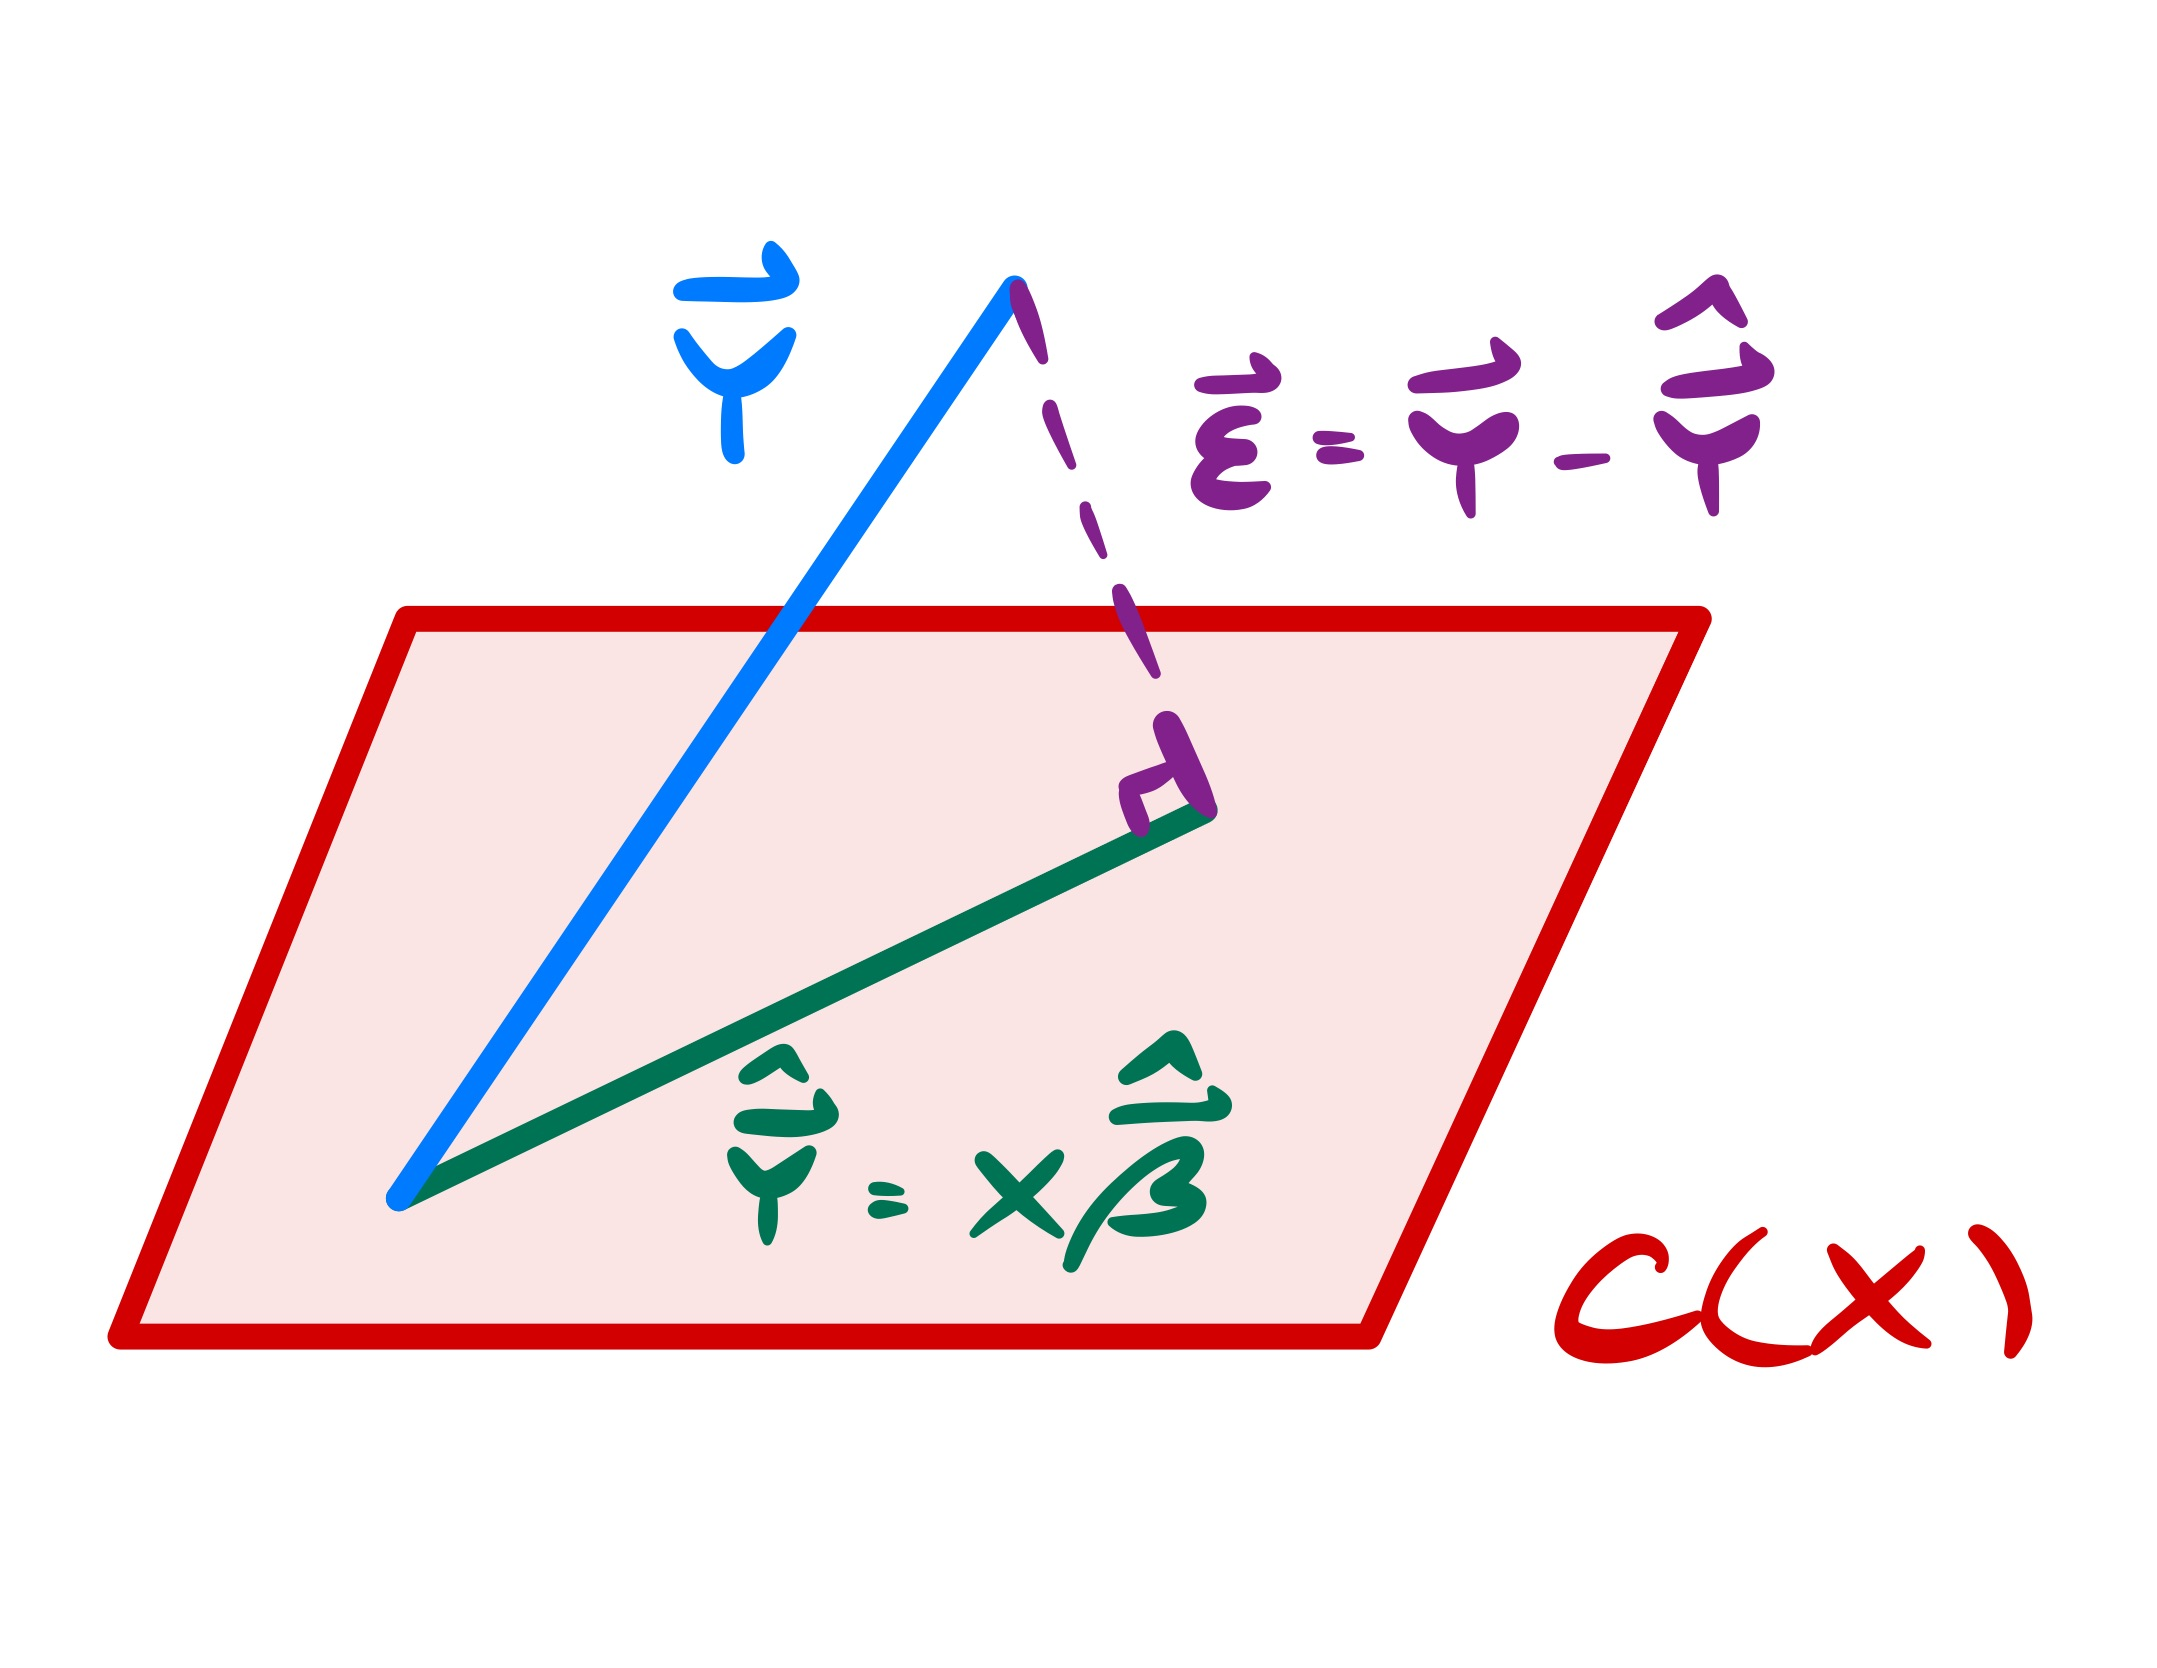
\includegraphics[width=0.5\textwidth]{stat139_section5_figure1.jpg}\\{\footnotesize FIGURE 1: The linear projection of $\vec{Y}$ onto $C(\boldsymbol{X})$.}
\end{center}

\begin{definition}[Orthogonality]
Two vectors $\vec{a}$ and $\vec{b}$ are \textit{orthogonal} if they are perpendicular to each other. Equivalently, \[\vec{a} \cdot \vec{b} = \vec{a}^{\top}\vec{b} = 0.\]
\end{definition}

\begin{definition}[Outcome and prediction vectors]
Let $\vec{Y}$ be the vector of \textit{outcomes} and let $\widehat{\vec{Y}} = \boldsymbol{X} \widehat{\vec{\beta}}$ be the vector of \textit{predictions}.

$\bullet$ Minimizing SSE is equivalent to getting $\widehat{\vec{Y}}$ as \textit{close} as possible to $\vec{Y}$.
\end{definition}

\begin{definition}[Residual vector]
Let $\vec{e} = \vec{Y} - \widehat{\vec{Y}}$ be the vector of \textit{residuals}.

$\bullet$ Minimizing SSE is equivalent to making $\vec{e}$ as \textit{small} as possible.
\end{definition}

\begin{definition}[Column space]
$C(\boldsymbol{X})$, the \textit{column space} of $\boldsymbol{X}$, is the set of all possible linear combinations of its column vectors.

$\bullet$ As a linear combination, $\widehat{\vec{Y}} = \boldsymbol{X} \widehat{\vec{\beta}}$ must reside in $C(\boldsymbol{X})$.

$\bullet$ Minimizing SSE is equivalent to finding the $\widehat{\vec{Y}} \in C(\boldsymbol{X})$ that is closest to $\vec{Y}$ in Euclidean distance—i.e., the $\ell_2$-norm of $\vec{e}$ is minimized.
\end{definition}

\begin{definition}[Linear projection]
Geometrically, the best $\widehat{\vec{Y}}$ is the \textit{linear projection} of $\vec{Y}$ onto $C(\boldsymbol{X})$.

$\bullet$ I.e., $\vec{e}$ is orthogonal to every column of $\boldsymbol{X}$, which implies that $\boldsymbol{X}^{\top} \vec{e} = 0$.
\end{definition}

\begin{definition}[OLS estimators]
We arrive at the same estimators: \[\widehat{\vec{\beta}}_{\OLS} = (\boldsymbol{X}^{\top} \boldsymbol{X})^{-1} \boldsymbol{X}^{\top} \vec{Y}.\footnote{See Appendix~\ref{app:ols-geom}.}\]
\end{definition}

% Section: Adding the Normality Assumption
\section{Adding the Normality Assumption}

\begin{idea}
Like before, the fifth assumption of Normality allows us to extend our inference.
\end{idea}

\subsection{Point Estimation for Parameters}

\begin{definition}[ELIHN]
Recall that the five main assumptions can be summarized as \[\varepsilon_i \simiid \N(0, \sigma^2),\] with $\sigma^2 < \infty$ for all $i \in \{1, \ldots, n\}$. In matrix notation, \[\vec{\varepsilon} \sim \MVN(\vec{0}, \sigma^2 I_{n \times n}),\] where $I_{n \times n}$ is the $n \times n$ identity matrix.

$\bullet$ Equivalently, \[Y_i \simind \N \left( \beta_0 + \sum_{j = 1}^{p} \beta_j x_{i, j}, \sigma^2 \right).\] In matrix notation, \[\vec{Y} \sim \MVN(\boldsymbol{X} \vec{\beta}, \sigma^2 I_{n \times n}).\]
\end{definition}

\begin{concept}
What does $\sigma^2 I_{n \times n}$ look like as a covariance matrix? What is on the diagonal elements? What is on the off-diagonal elements?
\end{concept}

\begin{solutionbox}
Visually, $\sigma^2 I_{n \times n} = 
\begin{pmatrix}
\sigma^2 & \ldots & 0 \\
\vdots & \ddots & \vdots \\
0 & \ldots & \sigma^2
\end{pmatrix}$, where each diagonal element is $\sigma^2$ while each off-diagonal element is $0$. This makes sense since, by assumption, each error is independent (implying $0$ covariance) and has the same variance.
\end{solutionbox}

\subsection{$t$-Based Inference for Parameters}

\begin{definition}[Distributions]
Under ELIHN, we have the following distributions for our estimators: \[\widehat{\vec{\beta}} \sim \MVN \left( \vec{\beta}, \sigma^2 (\boldsymbol{X}^{\top} \boldsymbol{X})^{-1} \right),\] \[\hat{\beta}_j \sim \N \left( \beta_j, \sigma^2 (\boldsymbol{X}^{\top} \boldsymbol{X})^{-1}_{(j + 1, j + 1)} \right),\] and \[\frac{n - (p + 1)}{\sigma^2} \hat{\sigma}^2_{\OLS} \sim \chi^2_{n - (p + 1)}\] for all $j \in \{0, \ldots, p\}$.
\end{definition}

\begin{definition}[Variance-covariance matrix]
From above, \[\Var[\widehat{\vec{\beta}}] = \sigma^2 (\boldsymbol{X}^{\top} \boldsymbol{X})^{-1},\] where $\sigma^2 (\boldsymbol{X}^{\top} \boldsymbol{X})^{-1}_{(j, k)}$ corresponds to row $j$ and column $k$ in the matrix—i.e., \[\sigma^2 (\boldsymbol{X}^{\top} \boldsymbol{X})^{-1}_{(j, k)} = \Cov[\hat{\beta}_{j - 1}, \hat{\beta}_{k - 1}].\]
\end{definition}

\begin{definition}[Hypothesis test for coefficient]
To test $H_0: \beta_j = 0$ vs. $H_A: \beta_j \neq 0$, we use \[T = \frac{\hat{\beta}_{j} - 0}{\hat{\sigma}_{\OLS} \sqrt{(\boldsymbol{X}^{\top} \boldsymbol{X})^{-1}_{(j + 1, j + 1)}}} \simnull t_{n - (p + 1)}\] as our \textit{test statistic} (i.e., its \textit{exact} distribution is known under $H_0$).
\end{definition}

\begin{definition}[Confidence interval for coefficient]
The $100(1 - \alpha)\%$ confidence interval for $\beta_j$ is \[\hat{\beta}_j \pm t_{1 - \frac{\alpha}{2}, n - (p + 1)} \times \hat{\sigma}_{\OLS} \sqrt{(\boldsymbol{X}^{\top} \boldsymbol{X})^{-1}_{(j + 1, j + 1)}}.\]
\end{definition}

\begin{concept}
In multiple linear regression, $\hat{\beta}_j \sim \N \left( \beta_j, \sigma^2 (\boldsymbol{X}^{\top} \boldsymbol{X})^{-1}_{(j + 1, j + 1)} \right)$. Show that this is equivalent to $\hat{\beta}_{1} \sim \N \left( \beta_1, \frac{\sigma^2}{s_{xx}} \right)$ in simple linear regression (where $p = 1$).
\end{concept}

\begin{solutionbox}
Let $p = 1$ and $j = 1$. By pattern-matching, we want to show that $\frac{\sigma^2}{s_{xx}} = \sigma^2 (\boldsymbol{X}^{\top} \boldsymbol{X})^{-1}_{(2, 2)} \iff \frac{1}{s_{xx}} = (\boldsymbol{X}^{\top} \boldsymbol{X})^{-1}_{(2, 2)}$. First, $\boldsymbol{X} = 
\begin{pmatrix}
1 & x_{1} \\
\vdots & \vdots \\
1 & x_{n}
\end{pmatrix}$, so $\boldsymbol{X}^{\top} \boldsymbol{X} = 
\begin{pmatrix}
1 & \ldots & 1 \\
x_{1} & \ldots & x_{n}
\end{pmatrix}
\begin{pmatrix}
1 & x_{1} \\
\vdots & \vdots \\
1 & x_{n}
\end{pmatrix} =
\begin{pmatrix}
n & \sum_{i = 1}^{n} x_{i} \\
\sum_{i = 1}^{n} x_{i} & \sum_{i = 1}^{n} x_{i}^2
\end{pmatrix}$. Since $\boldsymbol{X}^{\top} \boldsymbol{X}$ is a $2 \times 2$ matrix, $(\boldsymbol{X}^{\top} \boldsymbol{X})^{-1} = 
\frac{1}{n \sum_{i = 1}^{n} x_{i}^2 - (\sum_{i = 1}^{n} x_{i})^2}
\begin{pmatrix}
\sum_{i = 1}^{n} x_{i}^2 & - \sum_{i = 1}^{n} x_{i} \\
- \sum_{i = 1}^{n} x_{i} & n
\end{pmatrix}$, so $(\boldsymbol{X}^{\top} \boldsymbol{X})^{-1}_{(2, 2)} = \frac{1}{n \sum_{i = 1}^{n} x_{i}^2 - (\sum_{i = 1}^{n} x_{i})^2} (n)$, which simplifies to $\frac{1}{\sum_{i = 1}^{n} x_{i}^2 - \frac{1}{n} (\sum_{i = 1}^{n} x_{i})^2}$. Notice that $\sum_{i = 1}^{n} x_{i}^2 - \frac{1}{n} (\sum_{i = 1}^{n} x_{i})^2 = \sum_{i = 1}^{n} (x_i - \bar{x})^2$ by the sum of squares identity—i.e., $\sum_{i = 1}^{n} (x_i - c)^2 = \sum_{i = 1}^{n} (x_i - \bar{x})^2 + n(\bar{x} - c)^2$—with $c = 0$. Thus, $(\boldsymbol{X}^{\top} \boldsymbol{X})^{-1}_{(2, 2)} = \frac{1}{s_{xx}}$.
\end{solutionbox}

\subsection{Simple vs. Multiple Linear Regression}

\begin{center}
{
\scriptsize
\renewcommand{\arraystretch}{1.5}
\begin{tabular}{p{3.25cm}|p{6cm}|p{6cm}}
\textbf{Quantity} & \textbf{Simple Linear Regression} & \textbf{Multiple Linear Regression} \\ \hline

\textbf{Coefficient OLS Estimator's Distribution}
& Slope: $\hat{\beta}_{1} \sim \N \left( \beta_1, \frac{\sigma^2}{s_{xx}} \right)$, 

Intercept: $\hat{\beta}_{0} \sim \N \left( \beta_0, \sigma^2 \left( \frac{1}{n} + \frac{\bar{x}^2}{s_{xx}} \right) \right)$
& Joint: $\widehat{\vec{\beta}} \sim \MVN \left( \vec{\beta}, \sigma^2 (\boldsymbol{X}^{\top} \boldsymbol{X})^{-1} \right)$, 

Marginal: $\hat{\beta}_j \sim \N \left( \beta_j, \sigma^2 (\boldsymbol{X}^{\top} \boldsymbol{X})^{-1}_{(j + 1, j + 1)} \right)$ \\

\hline

\textbf{Variance OLS Estimator's Distribution}
& $\frac{n - 2}{\sigma^2} \hat{\sigma}^2_{\OLS} \sim \chi^2_{n - 2}$
& $\frac{n - (p + 1)}{\sigma^2} \hat{\sigma}^2_{\OLS} \sim \chi^2_{n - (p + 1)}$ \\

\hline

\textbf{Confidence Interval for Mean Response at $x_0$ or $\vec{x}_0 = (1, x_{0, 1}, \ldots, x_{0, p})^{\top}$}
& $(\hat{\beta}_{0} + \hat{\beta}_{1} x_0) \pm t_{1 - \frac{\alpha}{2}, n - 2} \times \hat{\sigma}_{\OLS} \sqrt{\frac{1}{n} + \frac{(x_0 - \bar{x})^2}{s_{xx}}}$
& $(\vec{x}_0^{\top} \widehat{\vec{\beta}}) \pm t_{1 - \frac{\alpha}{2}, n - (p + 1)} \times \hat{\sigma}_{\OLS} \sqrt{\vec{x_0}^{\top} (\boldsymbol{X}^{\top} \boldsymbol{X})^{-1} \vec{x_0}}$ \\
\hline

\textbf{Prediction Interval for New Response at $x_0$ or $\vec{x}_0 = (1, x_{0, 1}, \ldots, x_{0, p})^{\top}$}
& $(\hat{\beta}_{0} + \hat{\beta}_{1} x_0) \pm t_{1 - \frac{\alpha}{2}, n - 2} \times \hat{\sigma}_{\OLS} \sqrt{1 + \frac{1}{n} + \frac{(x_0 - \bar{x})^2}{s_{xx}}}$
& $(\vec{x}_0^{\top} \widehat{\vec{\beta}}) \pm t_{1 - \frac{\alpha}{2}, n - (p + 1)} \times \hat{\sigma}_{\OLS} \sqrt{1 + \vec{x_0}^{\top} (\boldsymbol{X}^{\top} \boldsymbol{X})^{-1} \vec{x_0}}$
\end{tabular}
}
\end{center}

\subsection{Contrast $t$-Tests}

\begin{definition}[Contrast $t$-test]
We can generalize the hypothesis test for a \textit{single coefficient}—instead, we're now interested in a \textit{linear combination of coefficients}.

$\bullet$ To test $H_0: \vec{c}^{\top} \vec{\beta} = \gamma_0$ vs. $H_A: \vec{c}^{\top} \vec{\beta} \neq \gamma_0$, we use \[T = \frac{\vec{c}^{\top} \widehat{\vec{\beta}} - \gamma_0}{\hat{\sigma}_{\OLS} \sqrt{\vec{c}^{\top} (\boldsymbol{X}^{\top} \boldsymbol{X})^{-1} \vec{c}}} \simnull t_{n - (p + 1)}\] as our \textit{test statistic} (i.e., its \textit{exact} distribution is known under $H_0$).
\end{definition}

\begin{concept}
We know that $\widehat{\vec{\beta}} \sim \MVN \left( \vec{\beta}, \sigma^2 (\boldsymbol{X}^{\top} \boldsymbol{X})^{-1} \right)$. Let $\Sigma = \sigma^2 (\boldsymbol{X}^{\top} \boldsymbol{X})^{-1}$. What is the distribution of $\vec{c}^{\top} \widehat{\vec{\beta}}$?
\end{concept}

\begin{solutionbox}
As a linear combination, $\vec{c}^{\top} \widehat{\vec{\beta}} \sim \N(\E[\vec{c}^{\top} \widehat{\vec{\beta}}], \Var[\vec{c}^{\top} \widehat{\vec{\beta}}])$. Specifically, $\E[\vec{c}^{\top} \widehat{\vec{\beta}}] = \vec{c}^{\top} \E[\widehat{\vec{\beta}}] = \vec{c}^{\top} \vec{\beta}$ by linearity and $\Var[\vec{c}^{\top} \widehat{\vec{\beta}}] = \vec{c}^{\top} \Sigma \vec{c}$ by quadratic form (see Problem 2 and Problem 3).
\end{solutionbox}

% \begin{concept}
% How can we use the contrast $t$-test to test the hypothesis test for a single coefficient (i.e., $H_0: \beta_j = 0$ vs. $H_A: \beta_j \neq 0$)?
% \end{concept}

% \begin{solutionbox}
% Let $\vec{c}$ equal 0 for all components except for the $(j + 1)$th component (corresponding to predictor $j$) and $\gamma_0 = 0$. This shows how the contrast $t$-test is a generalization of the standard hypothesis test.
% \end{solutionbox}

\begin{concept}
In the hypothesis test for a single coefficient, we see whether the change in expected outcome from a one-unit increase in a single predictor is significant. How can we use the contrast $t$-test to see whether the change in expected outcome from several predictors changing at once is significant? 
\end{concept}

\begin{solutionbox}
Recall that the model can be written as $\E[Y_i] = \beta_0 + \beta_1 x_{i, 1} + \ldots + \beta_p x_{i, p}$. We're interested in changing $x_{i, 1}, \ldots, x_{i, p}$ by some amounts $d_1, \ldots, d_p$. Let $\vec{c} = (0, d_1, \ldots, d_p)^{\top}$ and $\gamma_0 = 0$. This tests whether the specified simultaneous changes in predictors are associated with a nonzero change in the expected outcome—i.e., $H_0: d_1 \beta_1 + \ldots + d_p \beta_p = 0$ vs. $H_A: d_1 \beta_1 + \ldots + d_p \beta_p \neq 0$.
\end{solutionbox}

% Section: Practice Problems
\section{Practice Problems}

\begin{problem}
For this problem, refer to the code and output below.

(a) You're in the final round interview for your dream job, and you're asked to regress RFFT score on age and an indicator for smoking. But alas! You forget the code to produce a confidence interval. How can you impress your interviewers by recovering the $95\%$ confidence interval for $\beta_1$ from the output?

(b) Interpret the confidence interval.

(c) How does \texttt{Pr(>|t|):Age = <2e-16} provide a sanity check for your confidence interval?
\end{problem}

\begin{lstlisting}
```{r}
# Read df
df <- read.csv("./prevend.csv")

# Run linear regression model
model <- lm(RFFT ~ Age + Smoking, data = df)
summary(model)
```
\end{lstlisting}

\begin{routput}
Call:
lm(formula = RFFT ~ Age + Smoking, data = df)

Residuals:
    Min      1Q  Median      3Q     Max 
-69.878 -15.424  -0.979  14.392  78.060 

Coefficients:
             Estimate Std. Error t value Pr(>|t|)    
(Intercept) 134.58824    1.69799  79.263  < 2e-16 ***
Age          -1.18359    0.02994 -39.531  < 2e-16 ***
Smoking      -5.52078    0.79857  -6.913 5.47e-12 ***
---
Signif. codes:  0 '***' 0.001 '**' 0.01 '*' 0.05 '.' 0.1 ' ' 1

Residual standard error: 22.13 on 4092 degrees of freedom
Multiple R-squared:  0.278,	Adjusted R-squared:  0.2776 
F-statistic: 787.6 on 2 and 4092 DF,  p-value: < 2.2e-16
\end{routput}

\begin{solutionbox}
(a) Generally, for an estimator with an appropriate symmetric sampling distribution around the true parameter, the confidence interval for that parameter is in the form: $\text{estimator} \pm \text{critical value} \times \widehat{\SE}$. With $4092$ degrees of freedom, this $t$-distribution is very well approximated by a Standard Normal, so at $\alpha = 0.05$, we can use $z_{0.975} = 1.96$ as our critical value. Thus, our $95\%$ confidence interval for $\beta_1$ is $[-1.18359 - 1.96 \times 0.02994, -1.18359 + 1.96 \times 0.02994] = [-1.2422724, -1.1249076]$. More formally, we know that $T = \frac{\hat{\beta}_{j} - \beta_j}{\hat{\sigma}_{\OLS} \sqrt{(\boldsymbol{X}^{\top} \boldsymbol{X})^{-1}_{(j + 1, j + 1)}}} \sim t_{n - (p + 1)}$, so a $100(1 - \alpha)\%$ confidence interval for $\beta_1$ is in the form: $\hat{\beta}_{1} \pm t_{0.975, n - (2 + 1)} \times \hat{\sigma}_{\OLS} \sqrt{(\boldsymbol{X}^{\top} \boldsymbol{X})^{-1}_{(1 + 1, 1 + 1)}}$. Since $\hat{\beta}_1 \sim \N \left( \beta_1, \sigma^2 (\boldsymbol{X}^{\top} \boldsymbol{X})^{-1}_{(1 + 1, 1 + 1)} \right)$, its variance is $\Var[\hat{\beta}_{1}] = \sigma^2 (\boldsymbol{X}^{\top} \boldsymbol{X})^{-1}_{(1 + 1, 1 + 1)}$, so the estimator for its standard error is $\hat{\sigma}_{\OLS} \sqrt{(\boldsymbol{X}^{\top} \boldsymbol{X})^{-1}_{(1 + 1, 1 + 1)}}$.

(b) We are $95\%$ confident that $\beta_1$ is captured in the interval $[-1.2422724, -1.1249076]$, where $\beta_1$ is the change in expected RFFT score for each one-unit increase in age, holding smoking status constant. 

(c) The $p$-value assumes the null hypothesis that $H_0: \beta_1 = 0$. With such a low $p$-value, we have evidence to reject $H_0$. Our $95\%$ confidence interval is a range of plausible values for $\beta_1$, so it's reassuring that this range does not contain $0$.
\end{solutionbox}

\begin{problem}
% Let's practice using linear algebra to extend our knowledge from single-variable probability and statistics.
For an $n$-dimensional random vector $\vec{X}$, we define \[
\E[\vec{X}] = 
\begin{pmatrix}
\E[X_{1}] \\
\vdots \\
\E[X_{n}]
\end{pmatrix}, \ 
\Var[\vec{X}] = \E \left[ (\vec{X} - \E[\vec{X}])(\vec{X} - \E[\vec{X}])^{\top} \right].
\]

(a) Show that $\E[A \vec{X}] = A \E[\vec{X}]$ for any matrix $A$ and random vector $\vec{X}$.

(b) Show that $\Var[A \vec{X}] = A \Var[\vec{X}] A^{\top}$ for any matrix $A$ and random vector $\vec{X}$.

(c) For any matrix $A$ and vectors $\vec{x}$ and $\vec{y}$ of compatible dimensions, $\vec{x}^{\top} A \vec{y} = \vec{y}^{\top} A^{\top} \vec{x}$. Why?
\end{problem}

\begin{solutionbox}
(a) Without loss of generality, let $\vec{X}$ be $n$-dimensional and $A \in \R^{m \times n}$.

\[
A \vec{X} = 
\begin{pmatrix}
a_{1, 1} & \ldots & a_{1, n} \\
\vdots & \ddots & \vdots \\
a_{m, 1} & \ldots & a_{m, n}
\end{pmatrix}
\begin{pmatrix}
X_{1} \\
\vdots \\
X_{n}
\end{pmatrix} = 
\begin{pmatrix}
a_{1, 1} X_{1} + \ldots + a_{1, n} X_{n} \\
\vdots \\
a_{m, 1} X_{1} + \ldots + a_{m, n} X_{n}
\end{pmatrix}.
\]

\[
A \E[\vec{X}] = 
\begin{pmatrix}
a_{1, 1} & \ldots & a_{1, n} \\
\vdots & \ddots & \vdots \\
a_{m, 1} & \ldots & a_{m, n}
\end{pmatrix}
\begin{pmatrix}
\E[X_{1}] \\
\vdots \\
\E[X_{n}]
\end{pmatrix} = 
\begin{pmatrix}
a_{1, 1} \E[X_{1}] + \ldots + a_{1, n} \E[X_{n}] \\
\vdots \\
a_{m, 1} \E[X_{1}] + \ldots + a_{m, n} \E[X_{n}]
\end{pmatrix}.
\]

Notice that the $i$th entry of $A \vec{X}$—i.e., $(A \vec{X})_{i}$—is $a_{i, 1} X_{1} + \ldots + a_{i, n} X_{n}$ for all $i \in \{1, \ldots, m\}$. By linearity, $\E[(A \vec{X})_i] = \sum_{j = 1}^{n} a_{i, j} \E[X_{j}]$, which is exactly the same as the $i$th entry of $A \E[\vec{X}]$—i.e., $(A \E[\vec{X}])_{i}$. Thus, $\E[A \vec{X}] = A \E[\vec{X}]$.

(b) 
\[
\begin{aligned}
\Var[A \vec{X}] &= \E[(A \vec{X} - \E[A \vec{X}])(A \vec{X} - \E[A \vec{X}])^{\top}] && \text{by definition} \\
&= \E[(A \vec{X} - A \E[\vec{X}])(A \vec{X} - A \E[\vec{X}])^{\top}] && \text{by linearity} \\
&= \E[A(\vec{X} - \E[\vec{X}])(A(\vec{X} - \E[\vec{X}]))^{\top}] && \text{by factoring} \\
&= \E[A(\vec{X} - \E[\vec{X}])(\vec{X} - \E[\vec{X}])^{\top} A^{\top}] && \text{by transpose of a product} \\
&= A \E[(\vec{X} - \E[\vec{X}])(\vec{X} - \E[\vec{X}])^{\top}] A^{\top} && \text{by linearity} \\
&= A \Var[\vec{X}] A^{\top} && \text{by definition}
\end{aligned}
\]

(c) With compatible dimensions, $\vec{x} \in \R^{m \times 1}$ and $\vec{y} \in \R^{n \times 1}$. Note that $\vec{x}^{\top} A \vec{y}$ is a scalar since $\vec{x}^{\top} A \vec{y} = (\vec{x}^{\top} A) \vec{y}$ by associativity, and $\vec{x}^{\top} A \in \R^{1 \times n}$, so $(\vec{x}^{\top} A) \vec{y} \in \R$. A scalar is always equal to its transpose.

\[
\begin{aligned}
\vec{x}^{\top} A \vec{y} &= (\vec{x}^{\top} A \vec{y})^{\top} && \text{by transpose of a scalar} \\
&= \vec{y}^{\top} A^{\top} (\vec{x} ^{\top})^{\top} && \text{by transpose of a product} \\
&= \vec{y}^{\top} A^{\top} \vec{x} && \text{by transpose of a transpose}
\end{aligned}
\]
\end{solutionbox}

\begin{problem}
Put simply, a \textit{quadratic form} is an expression in the form $\vec{x}^{\top} A \vec{x}$, where $\vec{x}$ is a vector and $A$ is a square matrix. Let $\vec{X}$ be a random vector with $\Var[\vec{X}] = \Sigma$. Then, for any vector $\vec{a}$, \[\Var[\vec{a}^{\top} \vec{X}] = \vec{a}^{\top} \Sigma \vec{a},\] which is a quadratic form!

(a) A covariance matrix $\Sigma \in \R^{n \times n}$ must be positive semidefinite, meaning that \[\vec{a}^{\top} \Sigma \vec{a} \geq 0\] for all $\vec{a} \in \R^{n}$. Why?

(b) For simplicity, let $\vec{X} = (X_1, X_2)^{\top}$ and $\vec{a} = (a_1, a_2)^{\top}$. Find $\Var[a_1 X_1 + a_2 X_2]$ first by using single-variable probability and then by using linear algebra.
\end{problem}

\begin{solutionbox}
(a) Recall that variance can never be negative, so $\vec{a}^{\top} \Sigma \vec{a} = \Var[\vec{a}^{\top} \vec{X}] \geq 0$. Intuitively, $\vec{a}^{\top} \vec{X}$ corresponds to an arbitrary linear combination of the random variables, and $\vec{a}^{\top} \Sigma \vec{a}$ measures the variance of that linear combination.

(b) First, let's use single-variable probability:

\[
\begin{aligned}
\Var[a_1 X_1 + a_2 X_2] &= a_1^2 \Var[X_1] + a_2^2 \Var[X_2] + 2 a_1 a_2 \Cov[X_1, X_2] && \text{by bilinearity}
\end{aligned}
\]

Next, let's use linear algebra:

\[
\begin{aligned}
\Var[a_1 X_1 + a_2 X_2] &= \Var[\vec{a}^{\top} \vec{X}] && \text{by rewriting} \\
&= \vec{a}^{\top} \Sigma \vec{a} && \text{by quadratic form} \\
&= 
\begin{pmatrix}
a_1 & a_2
\end{pmatrix}
\begin{pmatrix}
\Var[X_1] & \Cov[X_1, X_2] \\
\Cov[X_1, X_2] & \Var[X_2]
\end{pmatrix}
\begin{pmatrix}
a_1 \\
a_2
\end{pmatrix} && \text{by substituting} \\
&= a_1^2 \Var[X_1] + a_2^2 \Var[X_2] + 2 a_1 a_2 \Cov[X_1, X_2] && \text{by matrix algebra}
\end{aligned}
\]
\end{solutionbox}

% \begin{problem}
% Consider the following model: \[\vec{Y} = \boldsymbol{X} \vec{\beta} + \vec{\varepsilon},\] where \[\vec{\varepsilon} \sim \MVN(\vec{0}, \Sigma)\] and $\Sigma$ is some arbitrary but valid covariance matrix (but one that is not necessarily equal to $\sigma^2 I$). Suppose that we naively use the ordinary least squares estimator: \[\widehat{\vec{\beta}}_{\OLS} = (\boldsymbol{X}^{\top} \boldsymbol{X})^{-1} \boldsymbol{X}^{\top} \vec{Y}.\] Thus, we ignore the true covariance structure of the errors.\footnote{Inspired by Questions 1 and 2 in \enquote{Final Practice Problems} by James Xenakis.}

% (a) Find $\Var[\widehat{\vec{\beta}}_{\OLS}]$ under the true model. Write your final expression in terms of $\boldsymbol{X}$ and $\Sigma$.

% (b) Now suppose that, instead of OLS, we use the generalized least squares (GLS) estimator, which correctly accounts for the true covariance structure of the errors: \[\widehat{\vec{\beta}}_{\GLS} = (\boldsymbol{X}^{\top} \Sigma^{-1} \boldsymbol{X})^{-1} \boldsymbol{X}^{\top} \Sigma^{-1} \vec{Y}.\] Find $\Var[\widehat{\vec{\beta}}_{\GLS}]$ under the true model. Write your final expression in terms of $\boldsymbol{X}$ and $\Sigma$.
% \end{problem}

% \begin{solutionbox}
% TBA
% \end{solutionbox}

% Appendix
\appendix
\section{Proofs}

\subsection{Geometric Derivation of OLS Estimators}
\label{app:ols-geom}

\begin{proof}
We want to show that $\widehat{\vec{\beta}}_{\OLS} = (\boldsymbol{X}^{\top} \boldsymbol{X})^{-1} \boldsymbol{X}^{\top} \vec{Y}$. We know that $\boldsymbol{X}^{\top} \vec{e} = 0$.

\[
\begin{aligned}
\boldsymbol{X}^{\top} \vec{e} = 0 &\implies \boldsymbol{X}^{\top} (\vec{Y} - \widehat{\vec{Y}}) = 0 && \text{since $\vec{e} = \vec{Y} - \widehat{\vec{Y}}$} \\
&\implies \boldsymbol{X}^{\top} (\vec{Y} - \boldsymbol{X} \widehat{\vec{\beta}}) = 0 && \text{since $\widehat{\vec{Y}} = \boldsymbol{X} \widehat{\vec{\beta}}$} \\
&\implies \boldsymbol{X}^{\top} \vec{Y} - \boldsymbol{X}^{\top} \boldsymbol{X} \widehat{\vec{\beta}} = 0 && 
\text{by distributing} \\
&\implies \boldsymbol{X}^{\top} \boldsymbol{X} \widehat{\vec{\beta}} = \boldsymbol{X}^{\top} \vec{Y} && 
\text{by adding $\boldsymbol{X}^{\top} \boldsymbol{X} \widehat{\vec{\beta}}$} \\
&\implies \widehat{\vec{\beta}} = (\boldsymbol{X}^{\top} \boldsymbol{X})^{-1} \boldsymbol{X}^{\top} \vec{Y} && 
\text{by multiplying by $(\boldsymbol{X}^{\top} \boldsymbol{X})^{-1}$}
\end{aligned}
\]
\end{proof}

\end{document}